\twocolumn[\colorsection{Transmisión del calor}]
\setcounter{figure}{0}
%
\begin{Exercise}
  \ifthenelse{\equal{\seleccionados}{true}}
  {\addToList{xyz-transmision}{\ExerciseHeaderNB}}{}
  Un extremo de una varilla metálica aislada se mantiene a $\SI{100}{\celsius}$, y el otro se mantiene a $\SI{0}{\celsius}$ con una mezcla de hielo y agua. La varilla tiene $\SI{60}{\centi\metre}$ de longitud y el área de su sección transversal es $\SI{1.25}{\square\centi\metre}$. El calor conducido por la varilla funde $\SI{8.5}{\gram}$ de hielo cada $\SI{10}{\minute}$. Calcule la conductividad térmica del metal.
\end{Exercise}
\begin{Answer}
  $\SI{227}{\watt.\metre^{-1}.\kelvin^{-1}}$
\end{Answer}
%
% \begin{Exercise}
%   A través de una ventana de vidrio de $\SI{1}{\square\metre}$ de área y $\SI{5}{\milli\metre}$ de espesor fluye calor a razón de $\SI{1600}{cal/\second}$, siendo la temperatura interior de $\SI{15}{\celsius}$ y la exterior de $\SI{25}{\celsius}$. Si la temperatura exterior aumenta a $\SI{35}{\celsius}$, ¿por cuál de las siguientes ventanas de área $A$ $\si{\square\metre}$ y espesor $w$ $\si{\milli\metre}$ la cambiaría para mantener el mismo flujo calórico?\\
% \begin{tabular*}{0.8\textwidth}{ccc}
%   \textit{a}) $A/w=0.40$ & \textit{b}) $A/w=0.13$ & \textit{c}) $A/w=0.20$\\
%   \textit{d}) $A/w=0.17$ & \textit{e}) $A/w=0.11$ & \textit{f}) $A/w=0.10$\\
% \end{tabular*}
% \end{Exercise}
% \begin{Answer}
%   Opción \textit{f})
% \end{Answer}
%
\begin{Exercise}
  Un método experimental para medir la conductividad térmica de un material aislante consiste en construir una caja del material y medir el aporte de potencia a un calentador eléctrico dentro de la caja, que mantiene el interior a una temperatura medida por encima de la temperatura de la superficie exterior. Suponga que en un aparato como el mencionado se requiere un aporte de potencia de $\SI{180}{\watt}$ para mantener la superficie interior de la caja $\SI{65.0}{\celsius}$ arriba de la temperatura de la superficie exterior. El área total de la caja es de $\SI{2.18}{\square\metre}$, y el espesor de la pared es de $\SI{3.90}{\centi\metre}$. Calcule la conductividad térmica del material en unidades del SI.
\end{Exercise}
\begin{Answer}
  $\SI{0.0495}{\watt.\metre^{-1}.\kelvin^{-1}}$
\end{Answer}
%
\begin{Exercise}\label{p:transmision00}
  \ifthenelse{\equal{\seleccionados}{true}}
  {\addToList{xyz-transmision}{\ExerciseHeaderNB}}{}
  En una casa se tiene una pared de ladrillos de $\SI{3}{\metre} \times \SI{4}{\metre}$, y espesor $\SI{15}{\centi\metre}$, que separa un ambiente a $\SI{25}{\celsius}$ del exterior a $\SI{5}{\celsius}$. Esta pared contiene una ventana que consiste en solo un panel de vidrio de $\SI{1.5}{\metre} \times \SI{1.5}{\metre} \times \SI{5}{\milli\metre}$. \textit{a}) Calcular la corriente de calor total a través del concreto y la ventana, sin incluir efectos de convección. \textit{b}) ¿Cuál es el porcentaje de calor que se pierde a través de la ventana respecto del total? \textit{c}) Repetir los cálculos para una situación donde la ventana es cubierta por una lámina de papel de espesor $\SI{0.750}{\milli\metre}$. \textit{Datos}: conductividad térmica del ladrillo = $\SI{0.6}{\watt.\metre^{-1}.\kelvin^{-1}}$; conductividad térmica del vidrio = $\SI{1}{\watt.\metre^{-1}.\kelvin^{-1}}$; conductividad térmica del papel = $\SI{0.050}{\watt.\metre^{-1}.\kelvin^{-1}}$.
\end{Exercise}
\begin{Answer}
	\begin{minipage}[t]{.4\textwidth}
    \textit{a}) $\SI{9780}{\watt}$\\ \textit{b}) 92\%\\ \textit{c}) $\SI{3030}{\watt}$ ($74.3$\%)
  \end{minipage}
\end{Answer}
%
%No se informan las conductividades, con la intención de que los estudiantes las busquen.
\begin{Exercise}
  \ifthenelse{\equal{\seleccionados}{true}}
  {\addToList{xyz-transmision}{\ExerciseHeaderNB}}{}
  Dos barras, una de latón y otra de cobre, están unidas extremo con extremo. La longitud de la barra de latón es $\SI{0.2}{\metre}$ y la de cobre es $\SI{0.8}{\metre}$. La sección transversal de cada segmento tiene un área de $\SI{0.005}{\square\metre}$. El extremo libre del segmento de latón está en contacto con agua hirviendo y el extremo libre del segmento de cobre se encuentra en contacto con una mezcla de hielo y agua, en ambos casos a presión atmosférica normal. Los lados de las varillas están aislados, por lo que no hay pérdida de calor a los alrededores. \textit{a}) ¿Cuál es la temperatura del punto en el que los segmentos de latón y de cobre se unen? \textit{b}) ¿Qué masa de hielo se funde en $\SI{5}{\minute}$ debido el calor conducido por la varilla compuesta?
\end{Exercise}
\begin{Answer}
	\begin{minipage}[t]{.4\textwidth}
    \textit{a}) $\SI{53.1}{\celsius}$; \textit{b}) $\SI{115}{\gram}$
  \end{minipage}
\end{Answer}
%
\begin{Exercise}\label{p:transmision02}
  El gráfico de la figura \ref{f:transmision02} representa la temperatura en función de la posición dentro de una barra cuya área transversal mide $\SI{3.00}{\centi\metre\squared}$ y su longitud total es $\SI{30}{\centi\metre}$. La barra está compuesta por dos materiales homogéneos, y conecta dos fuentes de calor a temperaturas constantes, transmitiendo $\SI{1.44}{cal/s}$. Determinar las conductividades térmicas de los materiales que forman la barra.
\end{Exercise}
\begin{Answer}
	\begin{minipage}[t]{.4\textwidth}
    $\SI{0.12}{cal/(cm.\celsius.s)}$ y $\SI{0.72}{cal/(cm.\celsius.s)}$
  \end{minipage}
\end{Answer}
%
\begin{center}
  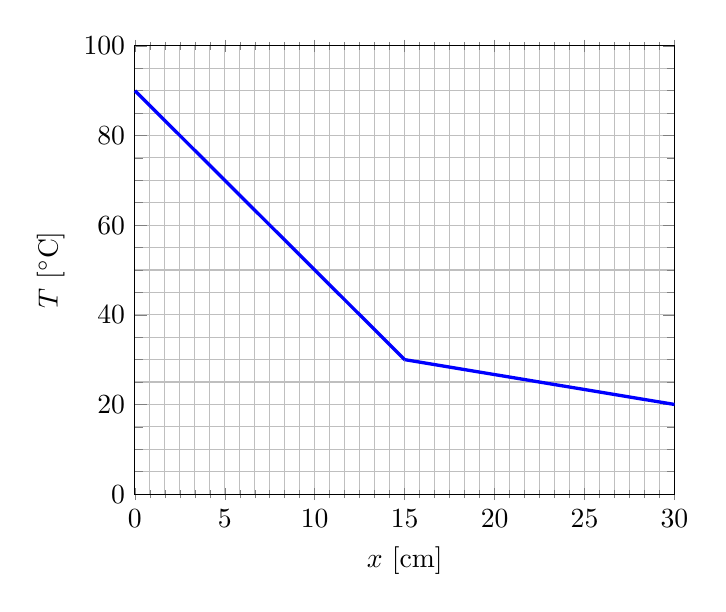
\begin{tikzpicture}[scale=1]
    \begin{axis}[
      % every major x tick/.append style={thick,blue},
      clip=false,
      grid=both,
      minor x tick num=5,
      minor y tick num=3,
      xmin=0, xmax=30,
      ymin=0, ymax=100,
      xtick  align=center,
      xlabel={$x$~[cm]},
      ylabel={$T$~[$^\circ$C]}
      ];
      \draw [color=blue, very thick](0,90)--(15,30);
      \draw [color=blue, very thick](15,30)--(30,20);
    \end{axis}
  \end{tikzpicture}
  \captionof{figure}{Problema \ref{p:transmision02}\label{f:transmision02}}
\end{center}
%
\begin{Exercise}
  Se sueldan varillas de cobre, latón y acero para formar una figura en forma de Y. El área de la sección transversal de cada varilla es de $\SI{2}{\square\centi\metre}$. El extremo libre de la varilla de cobre se mantiene a $\SI{100}{\celsius}$, y los extremos libres de las varillas de latón y acero a $\SI{0}{\celsius}$. Suponga que no hay pérdida de calor por los laterales de las varillas, cuyas longitudes son: $\SI{13}{\centi\metre}$, $\SI{18}{\centi\metre}$ y $\SI{24}{\centi\metre}$ para la de cobre, latón y acero respectivamente. \textit{a}) ¿Qué temperatura tiene el punto de unión? \textit{b}) Calcule la corriente de calor en cada una de las tres varillas.
\end{Exercise}
\begin{Answer}
	\begin{minipage}[t]{.4\textwidth}
    \textit{a}) $\SI{78.4}{\celsius}$\\ \textit{b}) $H_\text{latón} = \SI{9.50}{\watt}$, $H_\text{acero} = \SI{3.28}{\watt}$ y $H_\text{cobre} = \SI{12.8}{\watt}$
  \end{minipage}
\end{Answer}
%
\begin{Exercise}
  Una pared de ladrillos de $\SI{20}{\centi\metre}$ de espesor y conductividad térmica $\SI{5E-4}{cal/(\second.\centi\metre.\celsius)}$, separa una habitación en la que el aire está a una temperatura de $\SI{15}{\celsius}$, del exterior donde el aire se encuentra a una temperatura de $\SI{-5}{\celsius}$. Si el coeficiente de convección interior es de $\SI{1E-4}{cal/(\second.\centi\square\metre.\celsius)}$ y el doble de  éste en el exterior, calcular: \textit{a}) La temperatura de la superficie interior de la pared. \textit{b}) La temperatura de la superficie exterior de la pared.
\end{Exercise}
\begin{Answer}
  \begin{minipage}[t]{.4\textwidth}
    \textit{a}) $\SI{11.4}{\celsius}$\\ \textit{b}) $\SI{-3.16}{\celsius}$
  \end{minipage}
\end{Answer}
%
\begin{Exercise}\label{p:transmision01}
  Una pared exterior está compuesta por una capa externa de madera de $\SI{3.0}{\centi\metre}$ de espesor y una capa interna de espuma de poliestireno de $\SI{2.2}{\centi\metre}$ de espesor. Considere que la conductividad térmica de la madera es $k_\text{m} = \SI{0.08}{\watt.\metre^{-1}.\kelvin^{-1}}$ y la del poliestireno es $k_\text{p} = \SI{0.01}{\watt.\metre^{-1}.\kelvin^{-1}}$. La temperatura del aire en el interior es $\SI{19}{\celsius}$ y la del aire en el exterior es $\SI{-10}{\celsius}$, y los coeficientes de convección del aire en el interior y del aire en el exterior valen $\SI{5}{\watt/(\square\metre.\kelvin)}$ y $\SI{12}{\watt/(\square\metre.\kelvin)}$ respectivamente. \textit{a}) Calcular la rapidez del flujo de calor por metro cuadrado a través de esta pared. \textit{b}) Calcular la temperatura en la superficie de contacto entre la madera y la espuma de poliestireno. \textit{c}) Realizar un gráfico de la temperatura en función de la posición, en la dirección del flujo de calor.
\end{Exercise}
\begin{Answer}
	\begin{minipage}[t]{.4\textwidth}
    \textit{a}) $\SI{10.2}{\watt/\square\metre}$\\ \textit{b}) $\SI{-5.36}{\celsius}$
  \end{minipage}
\end{Answer}
%
\begin{Exercise}
  Un carpintero construye una cabaña rústica que tiene un piso de dimensiones $\SI{3.50}{\metre} \times \SI{3.00}{\metre}$. Sus paredes, que miden $\SI{2.50}{\metre}$ de alto y $\SI{1.80}{\centi\metre}$ de grosor, están hechas de una madera cuya conductividad térmica vale $\SI{0.517}{cal/(\hour.\centi\metre.\celsius)}$, y serán aisladas con un material sintético de conductividad térmica igual a $\SI{0.947}{cal/(\hour.\centi\metre.\celsius)}$. Se desea instalar una estufa que entregue una potencia calorífica de $\SI{1100}{kcal/\hour}$ para mantener el interior a una temperatura de $\SI{25.0}{\celsius}$ cuando la temperatura exterior es $\SI{2.00}{\celsius}$. Despreciando la pérdida de calor a través del techo y del piso, calcule el espesor mínimo necesario del material aislante. Considere que el  coeficiente de convección del aire $\SI{2.00E-4}{cal/(\second.\centi\square\metre.\celsius)}$ tanto en el interior como en el exterior.
\end{Exercise}
\begin{Answer}
  $\SI{0.51}{\centi\metre}$
\end{Answer}
%
\begin{Exercise}
  En un edificio de oficinas se está considerando reemplazar ventanas de un solo panel de vidrio de $\SI{3}{\milli\metre}$ de espesor por ventanas de doble panel de vidrio de $\SI{3}{\milli\metre}$ de espesor, separados por $\SI{5}{\milli\metre}$ de aire estanco. En ambos casos la conductividad térmica del vidrio es $\SI{1}{\watt/(\metre.\kelvin)}$ y en el caso de doble panel la conductividad térmica del aire estanco es $\SI{0.025}{\watt/(\metre.\kelvin)}$. El coeficiente de transmisión interior y exterior vale $\SI{20}{\watt/(\metre\squared.\kelvin)}$ y se puede despreciar la contribución por convección en el aire estanco. Las oficinas se calefaccionan con energía eléctrica cuyo costo es $\SI{116.63}{\$/kWh}$, para mantener la temperatura interior $\SI{10}{\celsius}$ por encima de la temperatura exterior, durante 220 horas mensuales. ¿Cuánto dinero se ahorrarían cada mes por cada metro cuadrado de ventana que se reemplace?
\end{Exercise}
\begin{Answer}
	\begin{minipage}[t]{.4\textwidth}
    \$ 1650
  \end{minipage}
\end{Answer}
%
\begin{Exercise}
  Calcule la tasa de radiación de energía por unidad de área de un cuerpo negro a: \textit{a}) $\SI{273}{\kelvin}$ y \textit{b}) $\SI{2730}{\kelvin}$.
\end{Exercise}
\begin{Answer}
	\begin{minipage}[t]{.4\textwidth}
    \textit{a}) $\SI{315}{\watt/\square\metre}$\\ \textit{b}) $\SI{3.15E6}{\watt/\square\metre}$
  \end{minipage}
\end{Answer}
%
\begin{Exercise}
  \ifthenelse{\equal{\seleccionados}{true}}
  {\addToList{xyz-transmision}{\ExerciseHeaderNB}}{}
  La emisividad del tungsteno es $0.350$. Una esfera de tungsteno con un radio de $\SI{1.5}{\centi\metre}$ se suspende dentro de una cavidad grande, cuyas paredes están a $\SI{290}{\kelvin}$. ¿Qué aporte de potencia se requiere para mantener la esfera a una temperatura de $\SI{3000}{\kelvin}$, si se desprecia la conducción de calor por los soportes?
\end{Exercise}
\begin{Answer}
  $\SI{4540}{\watt}$
\end{Answer}
%
\begin{Exercise}
  Calcular cuánto calor neto pierde cada hora una persona desnuda en forma de radiación, cuando se encuentra en un ambiente a $\SI{15}{\celsius}$. Suponer que la superficie libre que emite (y recibe) calor es de $\SI{2.5}{\metre\squared}$, su temperatura es $\SI{33}{\celsius}$, y se comporta como un cuerpo negro.
\end{Exercise}
\begin{Answer}
	\begin{minipage}[t]{.4\textwidth}
    $\SI{963}{\kilo\joule}$
  \end{minipage}
\end{Answer}
%
\begin{Exercise}
  La tasa de energía radiante que llega del Sol a la atmósfera superior de la Tierra es cercana a $\SI{1.5}{\kilo\watt/\square\metre}$. La distancia promedio de la Tierra al Sol es $\SI{1.5E11}{\metre}$ y el radio del Sol es $\SI{6.96E8}{\metre}$. \textit{a}) Calcule la tasa de radiación de energía por unidad de área de la superficie solar. \textit{b}) Si el Sol irradia como cuerpo negro ideal, ¿qué temperatura tiene en su superficie?
\end{Exercise}
\begin{Answer}
	\begin{minipage}[t]{.4\textwidth}
    \textit{a}) $\approx\SI{70}{\mega\watt/\square\metre}$\\ \textit{b}) $\approx\SI{5900}{\kelvin}$
  \end{minipage}
\end{Answer}
%